\chapter{Implementation}
\label{chap:implementation}
In this chapter, the implementation of the network stack using the
pipelined design from chapter \ref{chap:design} is outlined and described,
the application of SME detailed and evaluated, and lastly, the viability
of the system on an FPGA is discussed.\\
The network stack is implemented in C\# using the C\# version of SME, which is,
at the moment of writing, more mature and feature-rich. The current version of
the implementation supports most of the absolutely vital parts of the IPv4
protocol, as well as the UDP protocol, as specified by RFC 1122\cite{RFC1122}.
Although work has been carried out in order to ensure that additional protocols
can be implemented without obstructions, no additional protocols are supported
at the moment.\\
The solution is fairly well-divided into 3 different types of components,
relating closely to those of SME: processes, buffers, and busses. The most
interesting parts of these components will be described in further detail in the
following sections.


\section{Processes}
The processes are arguably the most vital part of the system, as they provide
the computation and "processing" on the in- and out-going packets.
It is important to note that although there are many other types of "processes",
in the network, such as the buffers, we will mainly refer to the modules doing
actual business-logic as "processes" \footnote{These processes are not to be
confused with SME processes, which are used for the implementation of both the
buffers and processes.}.

The essential processes in the network are represented as light-grey boxes in
the figure \ref{fig:final_design}. These processes are \texttt{Internet\_In},
\texttt{Internet\_Out}, and \texttt{Transport}.


\subsection{State-machines}
Network communication can consists of countless different packets, formats,
protocols, combinations of flags and settings, and even errors and corrupted
bits. The processes in the network have to take on a manifold of jobs in order
to handle all these scenarios, which sadly cannot be handled with a simple
combinational logic circuit. To operate under these various conditions, these
processes are modelled as finite state machines, maintaining a single state at
all times.\\
The processes have a lot of similar states, such as \texttt{Idle}, \texttt{Receive},
\texttt{Pass}, or \texttt{Send}, but these can work very differently, as shown
in the following sections. Before moving on to describing the state-machines of
the 3 processes, it is crucial to understand how these can be modelled in SME.

\subsubsection{SME process execution flow}
To implement a process in SME, the C\# class has to inherit from
either the \texttt{Process} abstract class, or the more simple
\texttt{SimpleProcess} class.
The latter class is, as its name states, a simpler version of the former. This
class implements an \texttt{OnTick()} method, which is invoked once for every
clock-cycle.\\
The more advanced, but also more capable \texttt{Process} class provides
an abstract method \texttt{Run} which is to be overriden and filled
with the code desired to be run in the process. The interesting feature
about this method is that it is asynchronous, meaning that the code can
execute other tasks while waiting for resources, such as functions,
to return. In this case, this asynchronous feature is used to give
the programmer ability to split the function into multiple segments,
separated by the clock signal.\\
Figure \ref{fig:example_fsm} compares these two approaches for the same
finite state-machine with 3 consequtive states.

The "synchronous" approach using a \texttt{SimpleProcess} in subfigure
\ref{fig:sme_example_process_sync_code} has to implement a
variable tracking the current state of the process. On each new clock, this
state has to be analysed and the inteded function to be called based on the
value. This approach requires a lot of approach and boilerplate code, especialy
if there are several states.\\
The asynchronous approach on subfigure
\ref{sme_example_process_async_code} on the other hand can do with only
single \texttt{Run()} method split into three parts -- A, B, and C.
After each code-segment, the process waits for the clock signal, and
continues with the execution of the next segment.  This functionality
gives the programmer a very granular control of the way a process
works, how it is split into multiple steps on the hardware, while
maintaining simplicity, as seen on the statemachine diagram on subfigure
\ref{fig:sme_example_process_fsm}.

\begin{figure*}
    \begin{subfigure}[b]{0.3\textwidth}
        \centering
\begin{lstlisting}[language={[Sharp]C}]
public class SomeProcess : StateProcess
{
  private override async Task OnTickAsync()
  {
    // A
    await ClockAsync();
    // B
    await ClockAsync();
    // C
    await ClockAsync();
  }
}
\end{lstlisting}
        \caption{Example using inheriting from \texttt{Process}, using the \texttt{Run()} asynchronous method.}
	\label{fig:sme_example_process_async_code}
    \end{subfigure}
\hfill
    \begin{subfigure}[b]{0.3\textwidth}
\begin{lstlisting}[language={[Sharp]C}]
public class SomeProcess : SimpleProcess
{
// Initial state
state = A;

protected override void OnTick()
{
  switch(state) {
    case A:
      a();
      state = B;
    case B:
      b();
      state = C;
    case C:
      c();
      state = A;
  }

}
\end{lstlisting}
	\caption{Example pseudocode of using a "synchronous" \texttt{SimpleProcess}}
	\label{fig:sme_example_process_sync_code}
    \end{subfigure}
\hfill
 \begin{subfigure}[b]{0.3\textwidth}
        \centering
        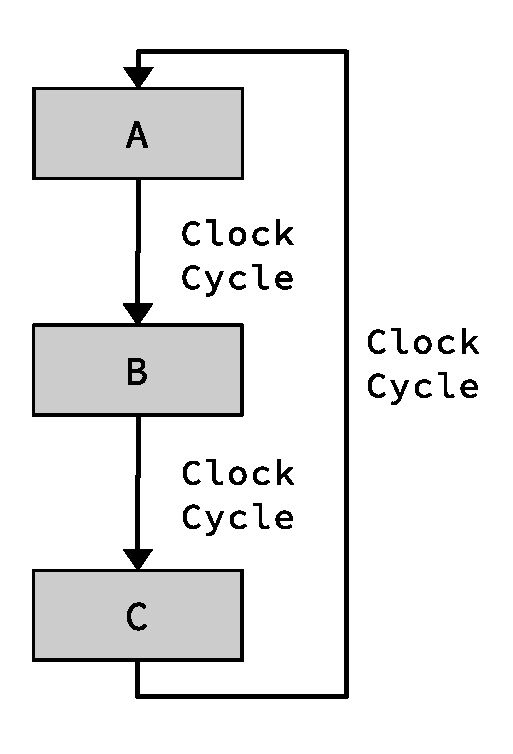
\includegraphics[scale=0.45]{implementation/empty_process_fsm.eps}
        \caption{The statemachine resulting from both code-examples}
 	\label{fig:sme_example_process_fsm}
\end{subfigure}
    \caption{A simple state-machine implemented in the asynchronous (left) and
asynchronous (right) approach in SME using C\#}
    \label{fig:example_fsm}
\end{figure*}


\subsubsection{\texttt{Internet Out} state machine}
This way of modelling a process in SME first the \texttt{Internet Out} process
very well, as it only has one responsibility, which is reading outgoing segments
and wrapping them in an Internet header. The figure \ref{fig:internet_out_implementation} shows the pseudo-code and state-machine for the \texttt{Internet Out}
process. This process was easy to model and implement, because it only has one
input and one output, and the state-changes are simple and intuitive.

\begin{figure*}[htpb]
    \centering
    \begin{subfigure}[b]{0.5\textwidth}
        \centering
\begin{lstlisting}[language={[Sharp]C}]
public partial class InternetOut: StateProcess
{
public override async Task OnTickAsync()
{
  while segment_available() {
    pass_segment();
    await ClockAsync();
  }

  while header_available() {
    pass_header();
    await ClockAsync();
  }
}
}
\end{lstlisting}
        \caption{Pseudo-code for the \texttt{InternetOut} process}
	\label{fig:internet_out_pseudocode}
    \end{subfigure}%
    \begin{subfigure}[b]{0.50\textwidth}
        \centering
        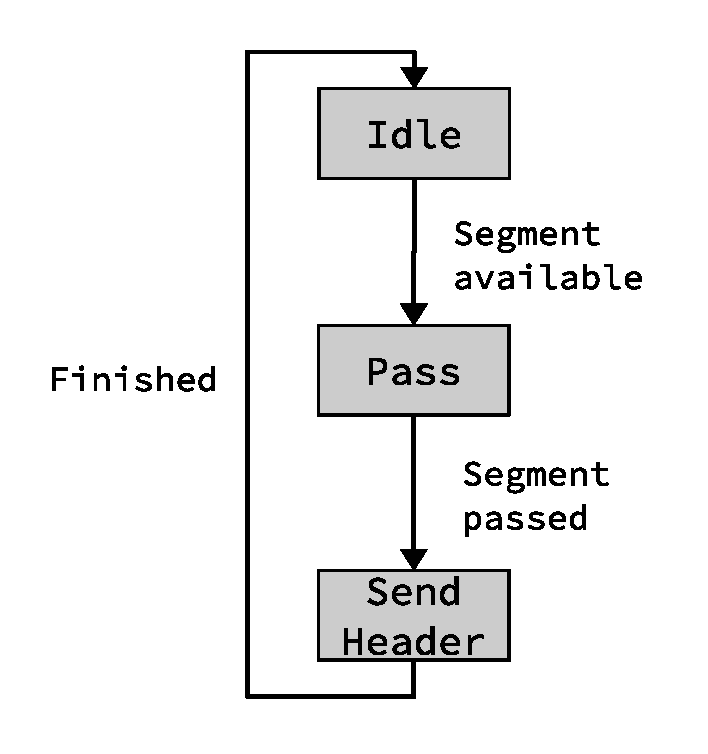
\includegraphics[scale=0.45]{implementation/internet_out_fsm.eps}
        \caption{The statemachine for the \texttt{InternetOut} process}
 	\label{fig:internet_out_fsm}
    \end{subfigure}%
    \caption{The implementation of the \texttt{InternetOut} process}
    \label{fig:internet_out_implementation}
\end{figure*}


\subsubsection{\texttt{Internet In} and \texttt{Transport} state machines}
Unfortunately,
The state-machine of \texttt{Internet In} is probably the most simple of all the
state-machines, as it can effectively only read new packets from the Link-layer,
and pass it along the pipeline. Although it might be desireable for the Internet
layer to send control packets out to the network, this is not supported in the
current build.



\begin{figure*}[t]
    \centering
    \begin{subfigure}[t]{0.5\textwidth}
        \centering
        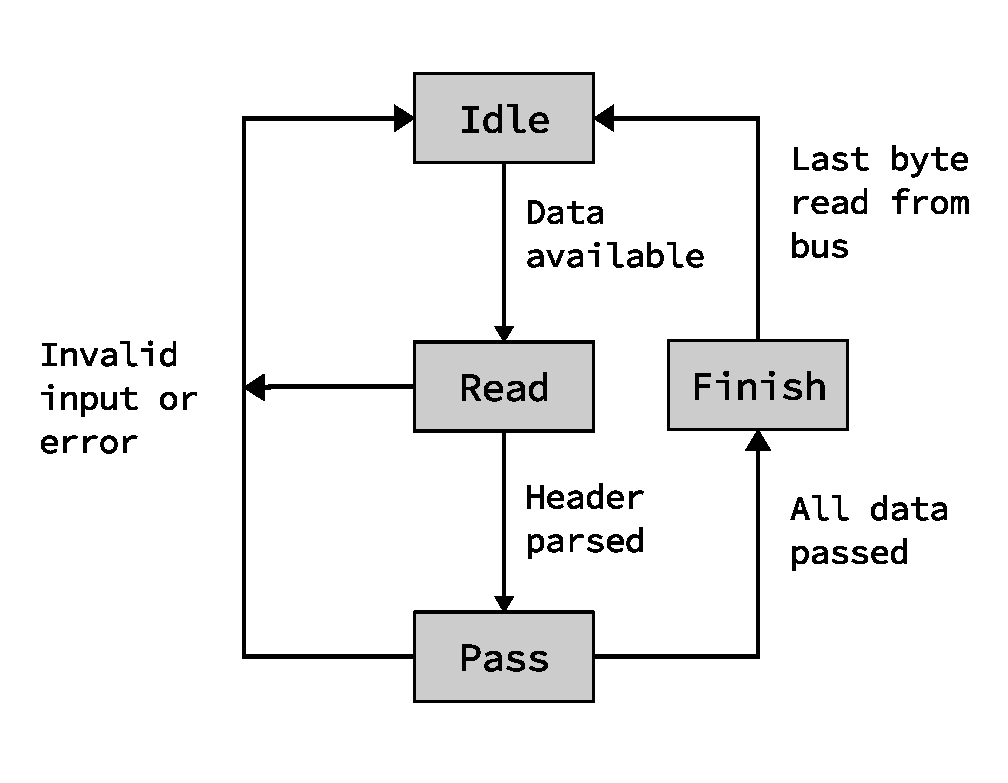
\includegraphics[scale=0.45]{implementation/internet_in_fsm.eps}
        \caption{The \texttt{Internet In} state machine}
    \end{subfigure}%
    \begin{subfigure}[t]{0.5\textwidth}
        \centering
        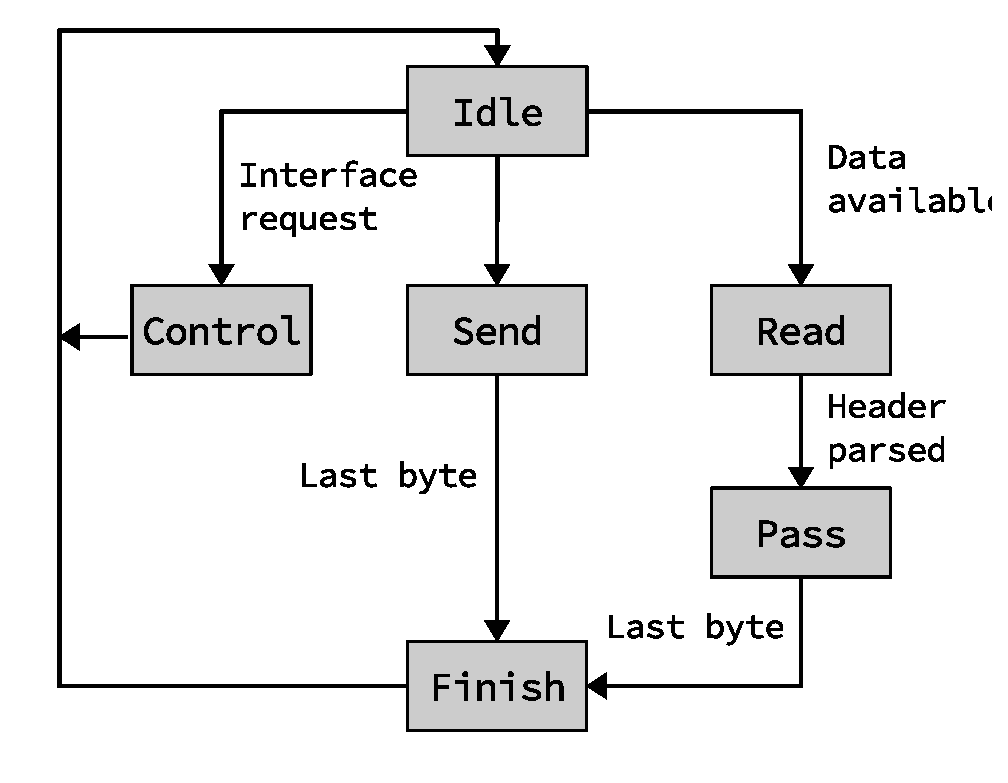
\includegraphics[scale=0.45]{implementation/transport_fsm.eps}
        \caption{The \texttt{Transport} state machine}
    \end{subfigure}%

    \caption{Statemachines for \texttt{Internet In} and \texttt{Transport}}
\end{figure*}

\subsubsection{\texttt{Internet Out} state machine}


\subsection{Internal memory}


\section{Buffers}
Problems such as packet fragmentation and out of order insertion are solved in
the memory buffers.\\
All of the buffers needs to handle input and output of
memory at the same time. If not, the system would slow down by a factor of two,
since the input would need to wait for the output to finish submitting, and
vice versa. This requires the underlying memory to handle read and write at the
same time. \\
Each of the memory buffers have slightly different variations. In general, there
are several problems to solve:

\begin{itemize}
    \item \textbf{Fragmentation}\\
    In \texttt{Segment In} and \texttt{Data In} there are segmentation. In
    \texttt{Segment In} IP segments may arrive out of order, and is therefore only
    sent through the system when all segments are received. \texttt{Data In} is
    essentially the same, just with other protocols such as TCP.\\
    In both cases we want the order to be concurrent. Packets that are not
    fragmented is in FIFO order. Fragmented packets in \texttt{Segment In} are
    held back, until all segments are received. Then all data segments are sent
    as a single block to \texttt{Transport}. In \texttt{Data In}, the segments are
    handled as a stream, where the last valid segment ID is known. The buffer
    only sends data when the last valid segment is set. This way, the buffer
    can contain segments with an higher ID than the valid, and know not to send it.


    \item \textbf{Unknown size}\\
    Some of the buffers do not get information about how much data has to be
    allocated. This happens in \texttt{Segment Out} and \texttt{Data Out}.
    In \texttt{Data Out} we do not know how much data the user sends into
    the system. (see: \autoref{subsubsec:interface_control}). In
    \texttt{Segment Out} we do not know some of the packet sizes, since
    \texttt{Transport} may not know how big the packet is going to be, for
    example when constructing an response packet.


    \item \textbf{Out-of-order submission}\\
    In Some cases the header of an packet can only be created after the data
    has been received. An example of this is the calculation of the checksum.\\
    This feature is required on \texttt{Frame Out} and \texttt{Frame Out}.
    This only applies to buffers where data is sent out and where calculations
    are done.

    \item \textbf{Data ready}\\
    When The buffer indicates that data is ready to be read, the next clock
    should also be ready and contain data. If not, the consumer would request
    data, wait at least 2 clocks for the data, and then request new data,
    slowing down the data transfer process significantly.

\end{itemize}
An oversight of this can be seen in \autoref{tab:buffer_requirements}.\\
\begin{table}[htpb]
  \begin{center}
      \begin{tabular}{l|c|c|c|c|}
          & \tablerot{Fragmentation}
          & \tablerot{\makecell{Unknown size}}
          & \tablerot{\makecell{Out-of-order \\ submission}}
          & \tablerot{\makecell{Data ready}} \\\hline
          \texttt{Frame Out}   &            &             & \checkmark & \checkmark \\ \hline
          \texttt{Segment In}  & \checkmark &             &            & \checkmark \\ \hline
          \texttt{Segment Out} &            & \checkmark  & \checkmark & \checkmark \\ \hline
          \texttt{Data In}     & \checkmark &             &            & \checkmark \\ \hline
          \texttt{Data Out}    &            & \checkmark  &            & \checkmark \\ \hline
      \end{tabular}
  \end{center}
  \caption{The requirements for the buffers} \label{tab:buffer_requirements}
\end{table}
\subsection{Components}
This section describes the components briefly to give a better overview of the
general structures of the buffers. The specific components are described in
detail in the following chapters.\\
To solve fragmentation the system uses "segments" in the memory.
A segment is an abstract structure consisting of metadata and two memory
addresses pointing to the start and end of the actual data.\\
To handle these segments, two interfaces are created, one to handle fixed size
allocations, and one to handle dynamic allocations, where the size is unknown.
Out-of-order submissions are solved simply by having an address sent beside the
data, which are added to the beginning of that respective segment.
See \autoref{subsec:memory_segments} for a in depth explanation.
\\
To keep order of the segments, a simple directory of keys and linked lists
are needed. The linked list are ordered at insertion time, so the fist element
always is the smallest. This makes lookup to the next element constant time, and
insertions of new at most $O(n)$ time. See \autoref{subsec:dictionary}.
\\
To have the data ready, a small internal buffer is needed. This small buffer
starts filling as soon as a segment is ready.
See \autoref{subsec:memory_types}.

\subsection{Memory segments} \label{subsec:memory_segments}
The memory segment structures consists of two types width slightly different
implementations. These are called Multi memory segments and Single memory
segments.
\\Their differences are explained in the end of this section.\\
Both types consists of an lookup table, where each table entry contains the
meta data and head and tail pointers. A Illustration of this can be seen in
\autoref{fig:memory_segments_explained}\\
In the implementation, the memory is not actually read, but an address is
returned. This makes it possible to use any memory type, since the latency issues
are in the submission and retrieval of the data itself, but not the calculations
for the address.\\
The lookup table consist of multiple segments references. A segment reference
contains meta data(Not illustrated in the figure) and a start and stop pointer.\\
In the illustration segments 0,1 and 4 are used, and 2 and 3 are free. Note that
segment 4 wraps around. If address 2 is requested from segment 4, memory address
15 is returned. If address 3 is requested, memory address 0 is returned.\\
\begin{figure}
	\centering
	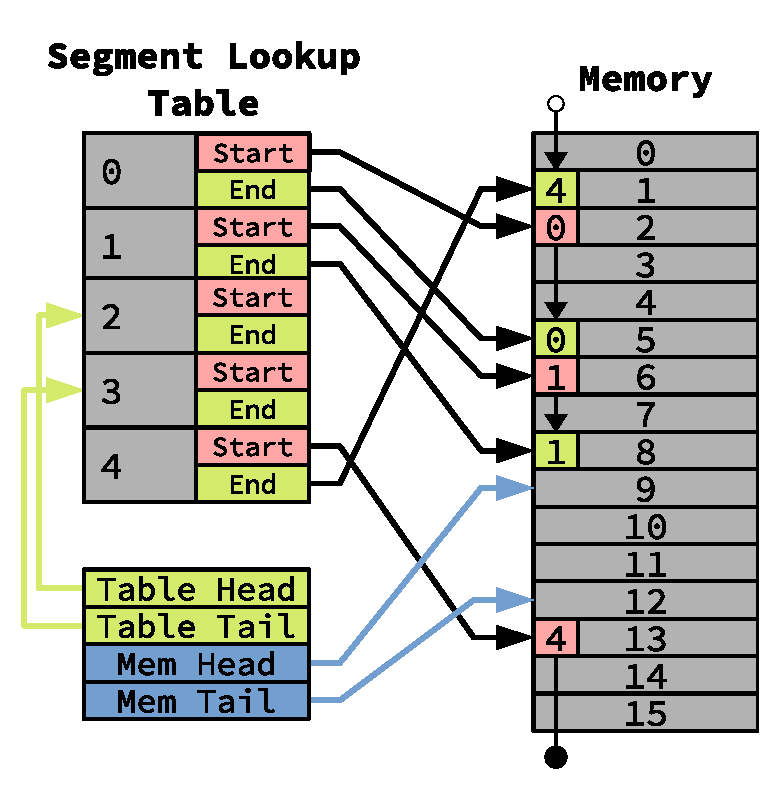
\includegraphics[width=\linewidth]{implementation/memory_segments.eps}
	\caption{The general structure of the memory segments in use.}
	\label{fig:memory_segments_explained}
\end{figure}

\subsubsection{Multi memory segments}
Each segment has three states, indicated by two boolean values; \texttt{Done}
and \texttt{Full}. When none are true, the segment is currently being filled
with data. When it is filled, and ready to be read, filled is marked as true,
and the data can now be read from. When the reading has ended, both \texttt{Done}
and \texttt{Full} are set to true, and the segment is now ready to be reused in
the lookup table. See \autoref{tab:memory_states_multi}.
\begin{table}[htpb]
  \begin{center}
      \begin{tabular}{l|c|c|}
          & \tablerot{\texttt{Full}}
          & \tablerot{\texttt{Done}} \\\hline
          \texttt{Filling}  &            &            \\ \hline
          \texttt{Reading}  & \checkmark &            \\ \hline
          \texttt{Done}     & \checkmark & \checkmark \\ \hline
      \end{tabular}
  \end{center}
  \caption{The memory states of "Multi memory segments"} \label{tab:memory_states_multi}
\end{table}
To describe the operation of the memory module, all the interface functions
are listed, and their operation explained.
The memory segment interface consists of the following functions:
\begin{description}
  \item[\mintinline{csharp}{int AllocateSegment(int size)}]\hfill\\
  When a segment is allocated, the new data is saved in the segment table
  head by looking at the \texttt{Table Head} pointer.\\
  The start and end pointers are calculated based on the \texttt{Mem Head}
  pointer. If the range between \texttt{Mem Head} and \texttt{Mem Tail} is
  smaller than \mintinline{csharp}{int size}, -1 is returned, indicating
  error. If not, the segment table id is
  returned(\mintinline{csharp}{int seg_ID}).

  \item[\mintinline{csharp}{int FocusSegment()}]\hfill\\
  A segment is classified as a focus segment if the data is ready to be sent
  (\texttt{Reading} state). It will automatically find the next segment, by
  increasing ... \notechange{Finish!}

  \item[\mintinline{csharp}{int SaveData(int seg_ID, int offset)}]\hfill\\
  Returns the memory address for that specific segment with an offset.
  This is calculated by finding the start address in the segment table, and
  adding the offset. If the segment is not in "Saving" state, an error
  is returned of -1.

  \item[\mintinline{csharp}{int LoadData(int seg_ID, int offset)}]\hfill\\
  The same as \mintinline{csharp}{int SaveData(...)}, with the exception
  that an error is returned if we are not in the loading state.

  \item[\mintinline{csharp}{int DelaySegment(int seg_ID)}]\hfill\\
  This function delays a focus segment by copying it to the table head

  \item[{\mintinline[breakanywhere]{csharp}{void SaveMetaData(int seg_ID, MetaData meta)}}]\hfill\\
    \noteerror{Fix overrunning item name}
  XXXX

  \item[\mintinline{csharp}{MetaData LoadMetaData(int seg_ID)}]\hfill\\
  XXXX
  \item[\mintinline{csharp}{void SegmentFull(int segment_ID)}]\hfill\\
  XXXX

  \item[\mintinline{csharp}{void SegmentDone(int segment_ID)}]\hfill\\
  XXXX

  \item[\mintinline{csharp}{int AllocateSegment(int size)}]\hfill\\
  XXXX
\end{description}

\subsubsection{Single memory segments}


\subsection{Dictionary} \label{subsec:dictionary}

\subsection{Memory types}  \label{subsec:memory_types}
Block ram on FPGA chips from companies such as Xilinx have a low latency, high
throughput but low capacity.\cite{xilinx_fpga_memory_resources}
The capacity limitation is a problem. Worst case the
system would have to hold multiple packets of the maximum size for that specific
protocol. For example, an \gls{ipv4} packet may have an max size of 65,535
bytes.\cite{RFC0791} If a lot of packets accumulate in the system, or the user
rarely empties the \texttt{Data In} buffer, we may run out of memory.\\
An additional solution would be the to use external memory with high latency,
low(or high) throughput and high capacity. The throughput would have to be equal
or bigger than the stream from the system itself, to not be an bottle neck.\\
In both cases, the memory takes at least one clock to get results back from
memory. To guarantee that the data is avaliable as soon as possible
(see: \autoref{sec:interface_signal_protocol}) one must use perfecting of the
memory.\\
This is solvable by using small internal buffers that use the fast registers.
The size of these small buffers would be based on the latency between the
request and response from memory. This would make it easier to
replace the underlying memory, by simply increasing the buffer size to that
of the memory latency.


\section{Interface Signal protocols}
\label{sec:interface_signal_protocol}
With the introduction of buffers between each parsing processes, a clear pattern
emerged. The layer-handling processes are responsible for numerous real-time tasks
(parsing, sending, protocol-specific tasks, etc), while also limited by their
fixed internal buffers. These processes are not always ready to receive input
from preceding processes, while they at the same time must be able to write their
output to following processes immediately.\\
The buffers are a stark opposite, as their large internal block memories enable
them to buffer huge chunks of memory, while also being able to wait for the
succeeding process to start reading.\\
With these two established scenarios, protocols for each can be proposed -- the
Buffer-Producer protocol, and the Compute-Producer protocol.

\subsection{Buffer-Producer}
The Buffer-Producer (BP) is the interface signal protocol where the producer of
the data is a buffer process (such as \texttt{Data Out} or \texttt{Segment
Out}).\\
The Buffer-Producer is heavily inspired by the Transfer signalling protocol in
the AXI4-Stream standard, which ensures a two-way flow-control mechanism for both
the producer and the consumer\footnote{The producer and consumer are called
master and slave respectively in the AXI4 specification.}\cite{arm_axi4}.

\begin{figure}[h]
\centering
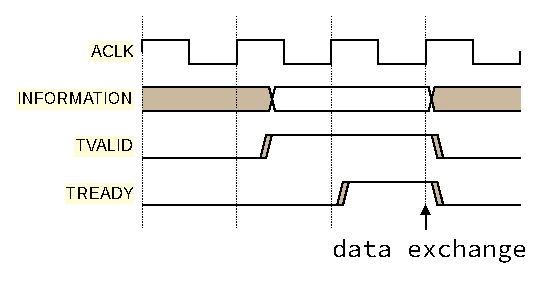
\includegraphics[scale=0.8]{implementation/axi4_handshake.eps}
\caption{The AXI4 handshake process, adapted from “AMBA 4 AXI4 Stream-Protocol
specification” by ARM, 2010, p. 19.}
\label{fig:axi4_handshake}
\end{figure}

The AXI4 protocol uses two signals (also called "flags"), the \texttt{TVALID}
on master, and \texttt{TREADY} on slave. Every time both \texttt{TVALID} and
\texttt{TREADY} are asserted during a clock-cycle, a data-exchange happens.
Figure \ref{fig:axi4_handshake} shows a data exchange, where the information
(the bytes) are placed on the bus and the \texttt{TVALID} is raised. When this
signal propagates to the slave, it asserts \texttt{TREADY}. When this signal
propagates back to the master, it knows that the information was read, and that
it can proceed with the next byte, or in this case, de-assert the
\texttt{TVALID} to indicate no more bytes available\cite{arm_axi4}.

The information transferred in the AXI4 protocol can be defined by the user,
but it usually is a payload consisting of multiple element, such as a byte
location or the type of the data.\\

The Buffer-Producer protocol draws heavy inspiration from this model, as it
provides a simple flow-protocol with only a few flags. In the BP protocol,
the producer has a \texttt{valid} flag, while the consumer has the
\texttt{ready} flag. However, without any modifications, the AXI4 protocol sees
the data exchanged as being a single data-stream.
In the case of the Buffer-Producer however, we want to differentiate between the
end of a packet (or simply just a segment of data), and the beginning of a new
one. In the very first iterations, this was done by distinguishing the parsed
data by finding a known delimiter, such as the ID of the IPv4 packet, or the
sequence number of the TCP header. Unfortunately, this solution is very
dependent on the scenario where different delimiters might appear, or not be
present at all. To generalize this issue, an additional signal
\texttt{bytes\_left} is added to the control bus of the protocol, which
indicates the end of a current data-block by setting \texttt{bytes\_left = 0}.
The final Buffer-Producer protocol can be summed up in these following rules:
\begin{itemize}
	\item A data transfer only occurs if both \texttt{valid} and \texttt{ready}
		are raised at the same clock-cycle.
	\item When the producer has data available, it is immediately put in
		the bus and the \texttt{valid} flag is raised.
	\item Once the \texttt{valid} flag is raised, it cannot be reset until
		a data-transfer occurs.
	\item The consumer is allowed to wait until the \texttt{valid} flag is
		raised before raising the \texttt{ready} flag.
	\item If a consumer raises the \texttt{ready} flag, it is allowed to
		reset it before \texttt{valid} is raised.
\end{itemize}

The conventional data-exchange using the BP protocol in the network
stack is perhaps better visualized by a sequence diagram on figure
\ref{fig:buffer_producer}.


\begin{figure}
	\centering
	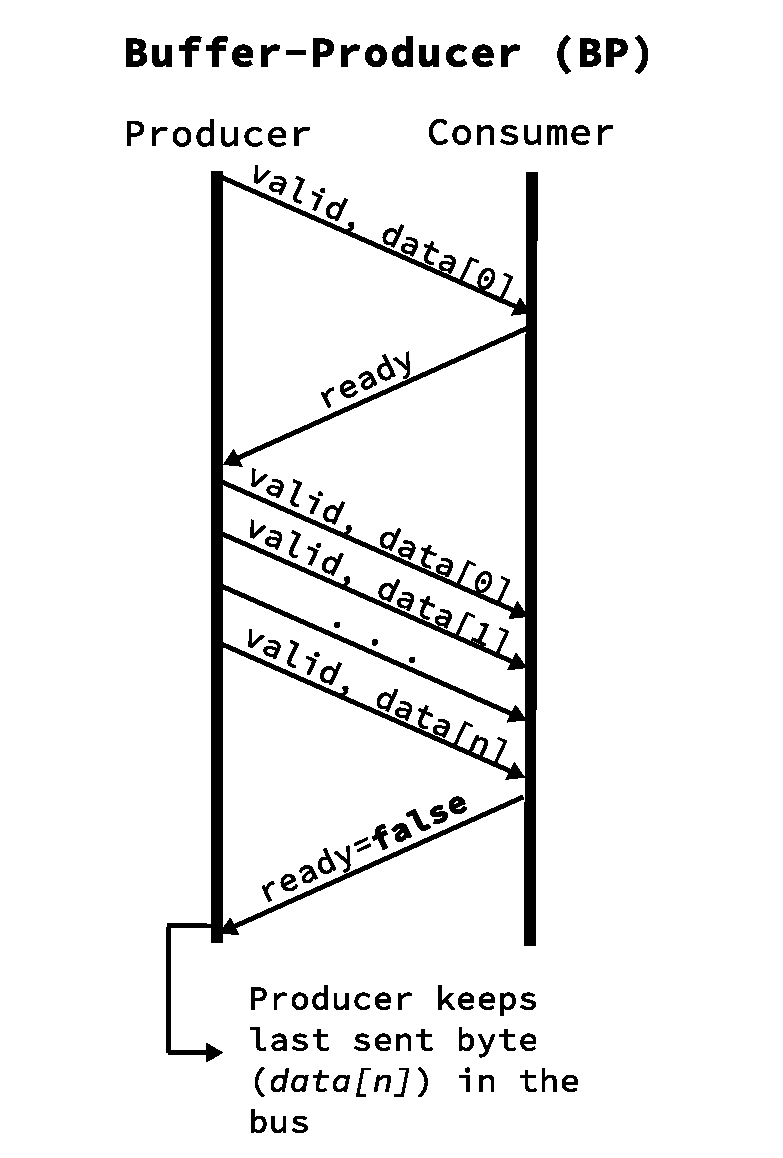
\includegraphics[scale=0.5]{implementation/buffer_producer.eps}
	\caption{The usual data-transfer between a buffer (Producer) and a
	compute-process (Consumer).}
	\label{fig:buffer_producer}
\end{figure}



\subsection{Compute-Producer}
The Compute-Producer (CP) protocol is the interface signal protocol from a
compute-process to a buffer. The requirement for this protocol is that
compute-processes do not usually have the luxury of being able to wait with the
data transfer, which usually happens if the compute-process is building a
packet header or passing information along from another buffer.

The concept for the Compute-Producer model is fairly simple; since the producer
(compute-process) does not have the luxury to wait, it always sends the data
on the bus, regardless if the consumer is ready. It is up to the producer to
mark the end of an ongoing data-stream.\\

Thus, the rules for the Compute-Producer protocol are as such:
\begin{itemize}
	\item If the producer puts data on the bus, the \texttt{valid} flag
		must be raised.
	\item If \texttt{bytes\_left} is greater than $0$, the data in the next
		clock will be valid.
	\item If \texttt{bytes\_left} is $0$, the current byte ends the
		current sequence of bytes.
	\item If the consumer deasserts \texttt{ready}, it \textit{may} not read the
		data in the bus.
	\item The producer may act upon the knowledge that the consumer is
		either reading (\texttt{ready = true}) or ignoring
		(\texttt{ready = false}) the data.
\end{itemize}

Such a scenario is visualized on figure \ref{fig:compute_producer}, where the
consumer becomes unavailable during the transaction. The producer has the
opportunity to drop the transaction, but it might also continue till the end.

\begin{figure}
	\centering
	\includegraphics[scale=0.5]{implementation/compute_producer.eps}
	\caption{The usual data-transfer between a compute-process (Producer) and a
	buffer (Consumer). Note that the consumer becomes unavailable halfway through the
	transaction.}
	\label{fig:compute_producer}
\end{figure}



\section{Interface Control}
The \texttt{Interface} is a collection of 3 busses provided to the user. Two of
the busses are direct connections to the data-buffer, used to transfer the
actual data to and from the network. As seen on \ref{fig:final_design}, the
connecting going to \texttt{Data In} follows the Compute-Producer interface
signal protocol, while the connection from \texttt{Data Out} follows the
Buffer-Producer protocol.\\
The connection going from the interface into the \texttt{Transport} process is
a bit more interesting. It is simply called the \texttt{InterfaceBus}, and it
is used to control the whole networking stack. As per usual, the connection
actually consists of a \texttt{InterfaceBus} controlled by the user, and the
\texttt{InterfaceControlBus}, used by the networking stack itself to respond to
the user requests.\\
Unlike the connection between buffers and processes where chunks of data are
transmitted over multiple clock-cycles, the interface connection is more of a
request-response model with only 1 clock-cycle required to submit the request
or send the response. However, after submitting the request, the user
\textit{should} keep the data in the bus until a response is received, because
the \texttt{Transport} process might be busy at the moment handling in- or
out-going packets, and not have time to process the request.\\
Figure \ref{fig:interfacebus_code} shows the definitions of the busses. Note
the \texttt{interface\_function} byte containing the type of "function" to
call, defined in the \texttt{InterfaceFunction enum} on figure
\ref{fig:interfacefunction_code}.


\begin{figure*}[t]
    \centering

    \begin{subfigure}[b]{0.45\textwidth}
	\centering
	 \begin{lstlisting}[language={[Sharp]C}]
enum InterfaceFunction : byte
{
    INVALID = 0,
//    BIND = 1,
    LISTEN = 2,
    CONNECT = 3,
    ACCEPT = 4,
    CLOSE = 7,
    // ...
    OPEN = 255,
}

struct InterfaceData
{
    public int socket;
    public uint ip;
    public byte protocol;
    public ushort port;
}\end{lstlisting}

        \caption{Definitions of the structures used in the interface busses}
	\label{fig:interfacefunction_code}
    \end{subfigure}
\hfill
    \begin{subfigure}[b]{0.45\textwidth}
	\centering
	 \begin{lstlisting}[language={[Sharp]C}]
interface InterfaceBus : IBus
{
    bool valid;
    byte interface_function;
    InterfaceData request;
}

interface InterfaceControlBus : IBus
{
    bool valid;

    byte exit_status;
    byte interface_function;
    InterfaceData request;
    InterfaceData response;
}\end{lstlisting}
	\caption{The definitions of the interface busses.}
	\label{fig:interfacebus_code}
    \end{subfigure}
    \caption{Pseudocode of the definitions used for the interface connection.}
	\label{fig:interface_definition}
\end{figure*}




\subsection{Usage}
The usage of this interface is very basic and primitive. The user sets the
appropriate values in the \texttt{InterfaceBus}, and raising the \texttt{valid}
flag. For example, to start listening on port $81$ using the \gls{udp}
protocol, the user would put these values in the bus:
\begin{Verbatim}[frame=single,samepage=true]
InterfaceBus {
  .interface_function = CONNECT
  .request {
    .ip = 10.0.0.2
    .protocol = UDP
    .port = 81
  }
  .valid = True
}
\end{Verbatim}
If the port is available under the \gls{udp} protocol and sockets are available
for allocation in the stack, the user should eventually receive a response.
Here, the user gets an \texttt{OK} response with the \texttt{socket = 2}:
\begin{Verbatim}[frame=single,samepage=true]
InterfaceControlBus {
  .valid = True
  .exit_status = OK
  .interface_function = CONNECT
  .request {
    .ip = 10.0.0.2
    .protocol = UDP
    .port = 81
  }
  .response {
    .socket = 2
  }
}
\end{Verbatim}

Once the user has received a valid socket, they can use the it at heart's
content for sending and receiving. For example, to send a byte:
\begin{Verbatim}[frame=single,samepage=true]
DataOut.WriteBus {
  .socket = 2
  .byte = "A"
}
DataOut.ComputeProducerBus {
  .valid = True
  .bytes_left = 0
}
\end{Verbatim}
The user is not required to wait for any response, as the Compute-Producer
interface signal protocol is used.


\subsection{Limitations}
As briefly mentioned, a big limitation of the interface control is that only
one request can be proposed at a time, and the user has to wait an arbitrary
number of clocks before the response arrives. The issue is that the
\texttt{Transport} might be occupied processing in-going and out-going
packets.\\
To circumvent this, experimental features of creating a queue of requests in
the \texttt{Transport}-process was made. However, this only added complexity to
the code, increased the resource-consumption of the process by a large margin
just in order to maintain the queue data-structure, and apart from convenience,
it added no improved performance. For these reasons, the initial approach was
kept.












